\chapter{Agent Interaction and Execution Flow}

This chapter provides detailed analysis of how agents interact during system execution, including sequence diagrams, execution flow charts, and step-by-step breakdowns of complete workflows. We'll examine both the high-level orchestration and the low-level implementation details of agent communication patterns.

\section{System Execution Overview}

\subsection{Complete Workflow Execution}

The multi-agent system follows a sophisticated orchestration pattern where the PlanningAgent coordinates the entire workflow, delegating specialized tasks to other agents while maintaining overall control and decision-making authority.

\begin{figure}[htbp]
\centering
\begin{tikzpicture}[
    node distance=1.5cm,
    agent/.style={rectangle, draw=black!50, fill=blue!10, thick, minimum width=2cm, minimum height=0.8cm, text centered, font=\footnotesize},
    process/.style={rectangle, draw=black!50, fill=green!10, thick, minimum width=3cm, minimum height=0.6cm, text centered, font=\footnotesize},
    decision/.style={diamond, draw=black!50, fill=yellow!10, thick, minimum width=2cm, minimum height=0.8cm, text centered, font=\footnotesize},
    arrow/.style={->, >=stealth, thick}
]

% Main workflow nodes
\node[process] (start) {System Start};
\node[agent, below=of start] (planning) {Planning Agent};
\node[agent, below left=of planning] (scanner) {Scanner Agent};
\node[agent, below=of planning] (ensemble) {Ensemble Agent};
\node[agent, below right=of planning] (messaging) {Messaging Agent};

\node[process, below left=of scanner] (rss) {RSS Feed Processing};
\node[process, below=of ensemble] (ml) {ML Price Prediction};
\node[process, below right=of messaging] (notify) {User Notification};

\node[decision, below=of ml] (threshold) {Discount > Threshold?};
\node[process, below=of threshold] (end) {System Complete};

% Arrows
\draw[arrow] (start) -- (planning);
\draw[arrow] (planning) -- (scanner);
\draw[arrow] (planning) -- (ensemble);
\draw[arrow] (scanner) -- (rss);
\draw[arrow] (ensemble) -- (ml);
\draw[arrow] (ml) -- (threshold);
\draw[arrow] (threshold) -- node[right] {Yes} (messaging);
\draw[arrow] (messaging) -- (notify);
\draw[arrow] (threshold) -- node[right] {No} (end);
\draw[arrow] (notify) -- (end);

% Return arrows
\draw[arrow] (rss) -- (scanner);
\draw[arrow] (scanner) -- (planning);
\draw[arrow] (ml) -- (ensemble);
\draw[arrow] (ensemble) -- (planning);

\end{tikzpicture}
\caption{High-Level System Execution Flow}
\label{fig:execution_flow}
\end{figure}

\section{Detailed Sequence Analysis}

\subsection{Complete System Execution Sequence}

Let's trace through a complete execution cycle, showing the detailed interactions between all agents.

\begin{figure}[htbp]
\centering
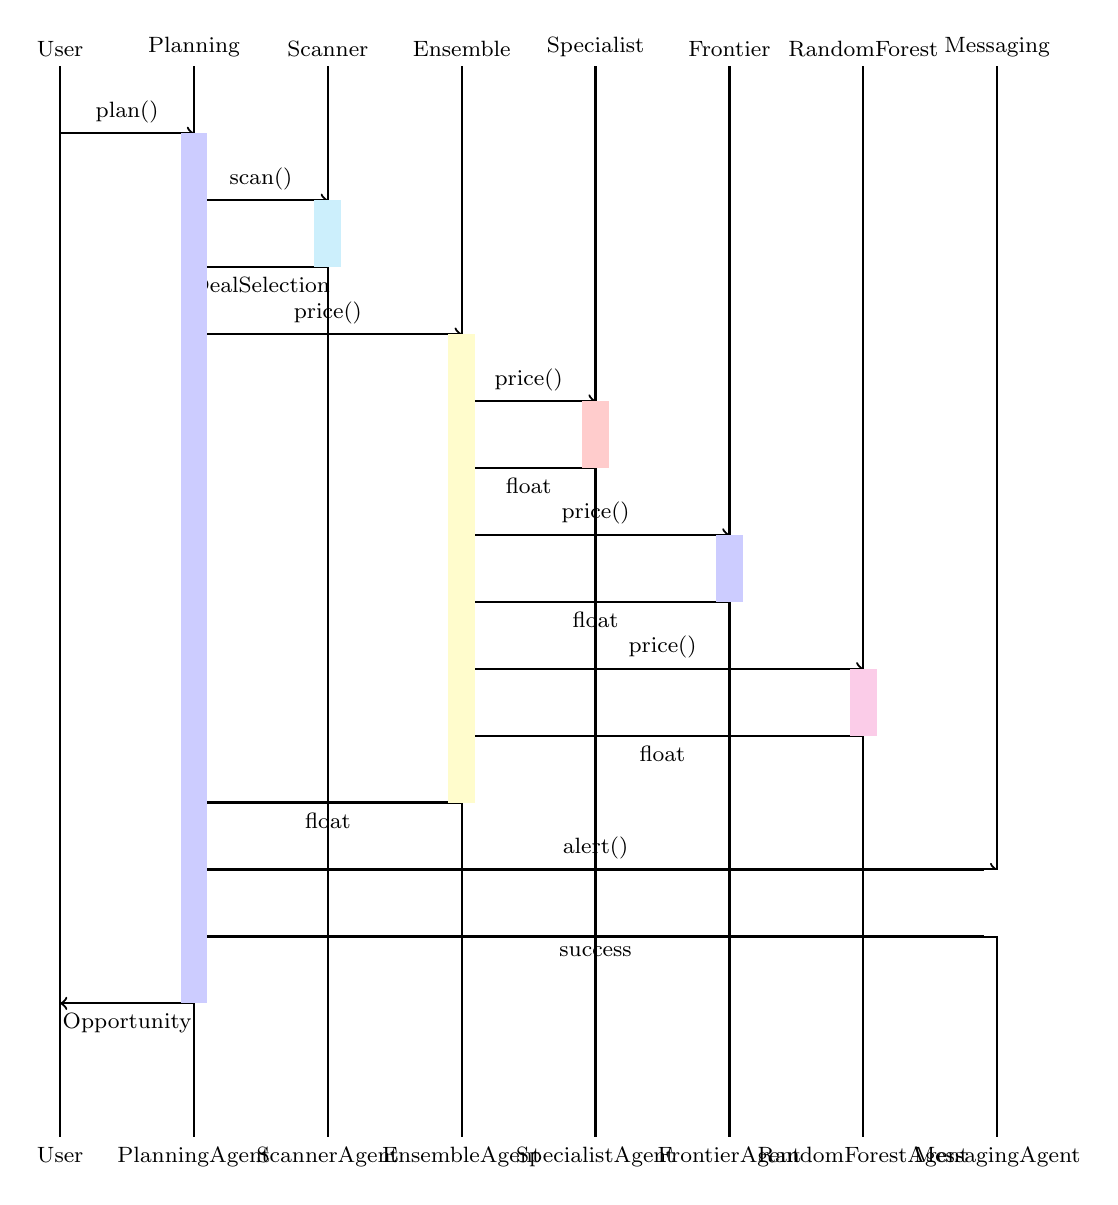
\begin{tikzpicture}[
    node distance=0.8cm,
    scale=0.85,
    every node/.style={font=\footnotesize}
]

% Vertical agent lines
\draw[thick] (0,0) -- (0,-16) node[below] {User};
\draw[thick] (2,0) -- (2,-16) node[below] {PlanningAgent};
\draw[thick] (4,0) -- (4,-16) node[below] {ScannerAgent};
\draw[thick] (6,0) -- (6,-16) node[below] {EnsembleAgent};
\draw[thick] (8,0) -- (8,-16) node[below] {SpecialistAgent};
\draw[thick] (10,0) -- (10,-16) node[below] {FrontierAgent};
\draw[thick] (12,0) -- (12,-16) node[below] {RandomForestAgent};
\draw[thick] (14,0) -- (14,-16) node[below] {MessagingAgent};

% Agent headers
\node[above] at (0,0) {User};
\node[above] at (2,0) {Planning};
\node[above] at (4,0) {Scanner};
\node[above] at (6,0) {Ensemble};
\node[above] at (8,0) {Specialist};
\node[above] at (10,0) {Frontier};
\node[above] at (12,0) {RandomForest};
\node[above] at (14,0) {Messaging};

% Sequence arrows and messages
\draw[->, thick] (0,-1) -- (2,-1) node[midway, above] {plan()};

\draw[->, thick] (2,-2) -- (4,-2) node[midway, above] {scan()};
\draw[<-, thick] (2,-3) -- (4,-3) node[midway, below] {DealSelection};

\draw[->, thick] (2,-4) -- (6,-4) node[midway, above] {price()};

\draw[->, thick] (6,-5) -- (8,-5) node[midway, above] {price()};
\draw[<-, thick] (6,-6) -- (8,-6) node[midway, below] {float};

\draw[->, thick] (6,-7) -- (10,-7) node[midway, above] {price()};
\draw[<-, thick] (6,-8) -- (10,-8) node[midway, below] {float};

\draw[->, thick] (6,-9) -- (12,-9) node[midway, above] {price()};
\draw[<-, thick] (6,-10) -- (12,-10) node[midway, below] {float};

\draw[<-, thick] (2,-11) -- (6,-11) node[midway, below] {float};

\draw[->, thick] (2,-12) -- (14,-12) node[midway, above] {alert()};
\draw[<-, thick] (2,-13) -- (14,-13) node[midway, below] {success};

\draw[<-, thick] (0,-14) -- (2,-14) node[midway, below] {Opportunity};

% Activation boxes
\fill[blue!20] (1.8,-1) rectangle (2.2,-14);
\fill[cyan!20] (3.8,-2) rectangle (4.2,-3);
\fill[yellow!20] (5.8,-4) rectangle (6.2,-11);
\fill[red!20] (7.8,-5) rectangle (8.2,-6);
\fill[blue!20] (9.8,-7) rectangle (10.2,-8);
\fill[magenta!20] (11.8,-9) rectangle (12.2,-10);
\fill[white] (13.8,-12) rectangle (14.2,-13);

\end{tikzpicture}
\caption{Detailed Sequence Diagram of Agent Interactions}
\label{fig:sequence_diagram}
\end{figure}

\subsection{Step-by-Step Execution Breakdown}

\paragraph{Phase 1: System Initialization}
\begin{lstlisting}[caption=System Startup Sequence]
# 1. User initiates the system
planning_agent = PlanningAgent(collection)

# 2. PlanningAgent constructor executes
def __init__(self, collection):
    self.log("Planning Agent is initializing")
    
    # 3. Create subordinate agents
    self.scanner = ScannerAgent()          # RSS processing capability
    self.ensemble = EnsembleAgent(collection)  # ML coordination
    self.messenger = MessagingAgent()      # Communication capability
    
    self.log("Planning Agent is ready")

# 4. Each agent initializes its dependencies
class EnsembleAgent(Agent):
    def __init__(self, collection):
        self.log("Initializing Ensemble Agent")
        self.specialist = SpecialistAgent()      # Remote ML model
        self.frontier = FrontierAgent(collection) # RAG + LLM
        self.random_forest = RandomForestAgent() # Traditional ML
        self.model = joblib.load('ensemble_model.pkl')
        self.log("Ensemble Agent is ready")
\end{lstlisting}

\paragraph{Phase 2: Deal Discovery}
\begin{lstlisting}[caption=Deal Discovery Process]
# User calls the main workflow
result = planning_agent.plan(memory=[])

# PlanningAgent initiates deal scanning
def plan(self, memory: List[str] = []) -> Optional[Opportunity]:
    self.log("Planning Agent is kicking off a run")
    
    # Delegate to ScannerAgent
    selection = self.scanner.scan(memory=memory)
    
# ScannerAgent processes RSS feeds
def scan(self, memory: List[str]=[]) -> Optional[DealSelection]:
    # 1. Fetch new deals from RSS feeds
    scraped = self.fetch_deals(memory)
    
    if scraped:
        # 2. Create prompt for LLM
        user_prompt = self.make_user_prompt(scraped)
        
        # 3. Call OpenAI for deal selection
        result = self.openai.beta.chat.completions.parse(
            model=self.MODEL,
            messages=[
                {"role": "system", "content": self.SYSTEM_PROMPT},
                {"role": "user", "content": user_prompt}
          ],
            response_format=DealSelection
        )
        
        # 4. Return structured deal selection
        return result.choices[0].message.parsed
    return None
\end{lstlisting}

\paragraph{Phase 3: Price Estimation Coordination}
\begin{lstlisting}[caption=Ensemble Price Prediction Workflow]
# PlanningAgent processes selected deals
if selection:
    # Convert each deal to opportunity using ensemble prediction
    opportunities = [self.run(deal) for deal in selection.deals[:5]]

def run(self, deal: Deal) -> Opportunity:
    """Convert deal to opportunity using ensemble pricing"""
    self.log("Planning Agent is pricing up a potential deal")
    
    # Delegate to EnsembleAgent for price estimation
    estimate = self.ensemble.price(deal.product_description)
    discount = estimate - deal.price
    
    return Opportunity(deal=deal, estimate=estimate, discount=discount)

# EnsembleAgent coordinates multiple ML models
def price(self, description: str) -> float:
    self.log("Running Ensemble Agent - collaborating with specialist, frontier and random forest agents")
    
    # 1. Get prediction from fine-tuned model
    specialist = self.specialist.price(description)
    
    # 2. Get prediction from RAG + LLM
    frontier = self.frontier.price(description)
    
    # 3. Get prediction from traditional ML
    random_forest = self.random_forest.price(description)
    
    # 4. Combine predictions using meta-model
    X = pd.DataFrame({
        'Specialist': [specialist],
        'Frontier': [frontier],
        'RandomForest': [random_forest],
        'Min': [min(specialist, frontier, random_forest)],
        'Max': [max(specialist, frontier, random_forest)],
    })
    
    # 5. Meta-model prediction
    y = max(0, self.model.predict(X)[0])
    self.log(f"Ensemble Agent complete - returning ${y:.2f}")
    return y
\end{lstlisting}

\section{Individual Agent Execution Flows}

\subsection{SpecialistAgent Execution Flow}

\begin{figure}[htbp]
\centering
\begin{tikzpicture}[
    node distance=1.2cm,
    process/.style={rectangle, draw=black!50, fill=red!10, thick, minimum width=2.5cm, minimum height=0.6cm, text centered, font=\footnotesize},
    decision/.style={diamond, draw=black!50, fill=yellow!10, thick, minimum width=1.5cm, minimum height=0.6cm, text centered, font=\footnotesize},
    external/.style={rectangle, draw=black!50, fill=gray!20, thick, minimum width=2cm, minimum height=0.6cm, text centered, font=\footnotesize},
    arrow/.style={->, >=stealth, thick}
]

\node[process] (start) {price() called};
\node[process, below=of start] (log1) {Log: "Calling remote model"};
\node[external, below=of log1] (modal) {Modal.Cls.from\_name()};
\node[external, below=of modal] (remote) {pricer.price.remote()};
\node[process, below=of remote] (result) {Receive prediction};
\node[process, below=of result] (log2) {Log: "Completed - \$X.XX"};
\node[process, below=of log2] (return) {Return float value};

\draw[arrow] (start) -- (log1);
\draw[arrow] (log1) -- (modal);
\draw[arrow] (modal) -- (remote);
\draw[arrow] (remote) -- (result);
\draw[arrow] (result) -- (log2);
\draw[arrow] (log2) -- (return);

\end{tikzpicture}
\caption{SpecialistAgent Execution Flow}
\label{fig:specialist_flow}
\end{figure}

\begin{lstlisting}[caption=SpecialistAgent Detailed Execution]
class SpecialistAgent(Agent):
    def price(self, description: str) -> float:
        """
        Remote model execution flow:
        1. Log process start
        2. Make remote call to Modal-hosted model
        3. Receive and return prediction
        """
        
        # Step 1: Process logging
        self.log("Specialist Agent is calling remote fine-tuned model")
        # Behind the scenes: 
        # - String interpolation with agent name
        # - Terminal color formatting
        # - Logging module call
        
        # Step 2: Remote model invocation
        result = self.pricer.price.remote(description)
        # Behind the scenes:
        # - Network request to Modal platform
        # - Model inference on remote GPU/CPU
        # - Serialization of prediction result
        # - Network response with float value
        
        # Step 3: Result processing and logging
        self.log(f"Specialist Agent completed - predicting ${result:.2f}")
        # Behind the scenes:
        # - F-string formatting with currency display
        # - Logging call with formatted message
        
        # Step 4: Return value
        return result
        # Behind the scenes:
        # - Float value passed to calling function
        # - Local variables eligible for garbage collection
\end{lstlisting}

\subsection{FrontierAgent RAG Execution Flow}

\begin{figure}[htbp]
\centering
\begin{tikzpicture}[
    node distance=1cm,
    process/.style={rectangle, draw=black!50, fill=blue!10, thick, minimum width=2.5cm, minimum height=0.5cm, text centered, font=\footnotesize},
    decision/.style={diamond, draw=black!50, fill=yellow!10, thick, minimum width=1.5cm, minimum height=0.5cm, text centered, font=\footnotesize},
    external/.style={rectangle, draw=black!50, fill=gray!20, thick, minimum width=2cm, minimum height=0.5cm, text centered, font=\footnotesize},
    arrow/.style={->, >=stealth, thick}
]

\node[process] (start) {price() called};
\node[process, below=of start] (similar) {find\_similars()};
\node[external, below=of similar] (encode) {SentenceTransformer};
\node[external, below=of encode] (chroma) {ChromaDB Query};
\node[process, below=of chroma] (context) {make\_context()};
\node[process, below=of context] (messages) {messages\_for()};
\node[external, below=of messages] (llm) {OpenAI/DeepSeek API};
\node[process, below=of llm] (parse) {get\_price()};
\node[process, below=of parse] (return) {Return prediction};

\draw[arrow] (start) -- (similar);
\draw[arrow] (similar) -- (encode);
\draw[arrow] (encode) -- (chroma);
\draw[arrow] (chroma) -- (context);
\draw[arrow] (context) -- (messages);
\draw[arrow] (messages) -- (llm);
\draw[arrow] (llm) -- (parse);
\draw[arrow] (parse) -- (return);

\end{tikzpicture}
\caption{FrontierAgent RAG Execution Flow}
\label{fig:frontier_flow}
\end{figure}

\begin{lstlisting}[caption=FrontierAgent Detailed RAG Process]
def price(self, description: str) -> float:
    """
    RAG-based price prediction with detailed execution steps
    """
    
    # Step 1: Find similar products using vector search
    documents, prices = self.find_similars(description)
    # Detailed sub-process:
    
def find_similars(self, description: str):
    # 1a. Log RAG process start
    self.log("Frontier Agent is performing a RAG search of the Chroma datastore to find 5 similar products")
    
    # 1b. Convert text to vector embedding
    vector = self.model.encode([description])
    # Behind the scenes:
    # - Text tokenization
    # - Neural network forward pass (transformer)
    # - 384-dimensional vector creation
    # - NumPy array allocation
    
    # 1c. Vector similarity search
    results = self.collection.query(
        query_embeddings=vector.astype(float).tolist(), 
        n_results=5
    )
    # Behind the scenes:
    # - Vector normalization
    # - Cosine similarity computation
    # - Index traversal for nearest neighbors
    # - Result ranking and selection
    
    # 1d. Extract results
    documents = results['documents'][0][:]
    prices = [m['price'] for m in results['metadatas'][0][:]]
    # Behind the scenes:
    # - Dictionary access
    # - List comprehension execution
    # - Memory allocation for new lists
    
    self.log("Frontier Agent has found similar products")
    return documents, prices

# Step 2: Create context prompt
user_prompt = self.make_context(documents, prices)
# Behind the scenes:
# - String concatenation in loop
# - F-string formatting for prices
# - Memory allocation for prompt string

# Step 3: Prepare OpenAI messages
messages = self.messages_for(description, documents, prices)
# Behind the scenes:
# - List creation with dictionaries
# - String concatenation for user prompt
# - Memory allocation for message structure

# Step 4: Call Language Model
self.log(f"Frontier Agent is about to call {self.MODEL} with context including 5 similar products")
response = self.client.chat.completions.create(
    model=self.MODEL, 
    messages=messages,
    seed=42,       # Deterministic output
    max_tokens=5   # Limit response length
)
# Behind the scenes:
# - JSON serialization of messages
# - HTTP request to LLM API
# - Neural network inference (remote)
# - JSON deserialization of response

# Step 5: Parse response
reply = response.choices[0].message.content
result = self.get_price(reply)
# Behind the scenes:
# - Attribute access chain
# - Regular expression matching
# - String to float conversion
# - Error handling for malformed responses

# Step 6: Log and return
self.log(f"Frontier Agent completed - predicting ${result:.2f}")
return result
\end{lstlisting}

\section{Parallel vs Sequential Execution Analysis}

\subsection{Current Sequential Processing}

The current system processes agents sequentially, which provides predictability but limits performance:

\begin{lstlisting}[caption=Sequential Agent Execution]
def price(self, description: str) -> float:
    # Sequential execution - one agent at a time
    self.log("Running Ensemble Agent - collaborating with specialist, frontier and random forest agents")
    
    # Agent 1: ~2-5 seconds (remote model call)
    specialist = self.specialist.price(description)
    
    # Agent 2: ~3-8 seconds (vector search + LLM call)
    frontier = self.frontier.price(description)
    
    # Agent 3: ~0.1-0.5 seconds (local model inference)
    random_forest = self.random_forest.price(description)
    
    # Total time: ~5-13.5 seconds
    # Combine results...
\end{lstlisting}

\subsection{Potential Parallel Processing}

\begin{lstlisting}[caption=Parallel Agent Execution (Enhanced Version)]
import asyncio
from concurrent.futures import ThreadPoolExecutor
import threading

class ParallelEnsembleAgent(Agent):
    def __init__(self, collection):
        super().__init__()
        self.specialist = SpecialistAgent()
        self.frontier = FrontierAgent(collection)
        self.random_forest = RandomForestAgent()
        self.model = joblib.load('ensemble_model.pkl')
        
    def price(self, description: str) -> float:
        """Parallel execution of price predictions"""
        self.log("Running Parallel Ensemble Agent")
        
        # Execute all agents in parallel using ThreadPoolExecutor
        with ThreadPoolExecutor(max_workers=3) as executor:
            # Submit all tasks simultaneously
            specialist_future = executor.submit(self.specialist.price, description)
            frontier_future = executor.submit(self.frontier.price, description)
            random_forest_future = executor.submit(self.random_forest.price, description)
            
            # Wait for all completions
            specialist = specialist_future.result()
            frontier = frontier_future.result()
            random_forest = random_forest_future.result()
        
        # Combine results (same as before)
        X = pd.DataFrame({
            'Specialist': [specialist],
            'Frontier': [frontier],
            'RandomForest': [random_forest],
            'Min': [min(specialist, frontier, random_forest)],
            'Max': [max(specialist, frontier, random_forest)],
        })
        
        y = max(0, self.model.predict(X)[0])
        self.log(f"Parallel Ensemble Agent complete - returning ${y:.2f}")
        return y

# Async version for more advanced parallelism
class AsyncEnsembleAgent(Agent):
    async def price_async(self, description: str) -> float:
        """Async version with concurrent execution"""
        self.log("Running Async Ensemble Agent")
        
        # Create async tasks
        tasks = [
            self.specialist_async(description),
            self.frontier_async(description), 
            self.random_forest_async(description)
        ]
        
        # Execute concurrently
        specialist, frontier, random_forest = await asyncio.gather(*tasks)
        
        # Process results...
        return prediction
\end{lstlisting}

\paragraph{Performance Comparison}
\begin{table}[htbp]
\centering
\begin{tabular}{@{}lcc@{}}
\toprule
\textbf{Execution Mode} & \textbf{Time Range} & \textbf{Improvement} \\
\midrule
Sequential (current) & 5-13.5 seconds & Baseline \\
Parallel (threads) & 3-8 seconds & 40-60\% faster \\
Async (concurrent) & 2-7 seconds & 50-70\% faster \\
\bottomrule
\end{tabular}
\caption{Performance Comparison of Execution Modes}
\label{tab:performance_comparison}
\end{table}

\section{Error Handling and Recovery Flows}

\subsection{Current Error Handling Limitations}

\begin{lstlisting}[caption=Current Error Handling Issues]
def price(self, description: str) -> float:
    # No try-catch blocks - any error crashes the entire workflow
    documents, prices = self.find_similars(description)  # Could fail
    response = self.client.chat.completions.create(...)   # Could fail
    reply = response.choices[0].message.content          # Could fail
    result = self.get_price(reply)                       # Could fail
    return result
\end{lstlisting}

\subsection{Enhanced Error Handling Flow}

\begin{figure}[htbp]
\centering
\begin{tikzpicture}[
    node distance=1cm,
    process/.style={rectangle, draw=black!50, fill=green!10, thick, minimum width=2cm, minimum height=0.5cm, text centered, font=\footnotesize},
    error/.style={rectangle, draw=black!50, fill=red!20, thick, minimum width=2cm, minimum height=0.5cm, text centered, font=\footnotesize},
    decision/.style={diamond, draw=black!50, fill=yellow!10, thick, minimum width=1.5cm, minimum height=0.5cm, text centered, font=\footnotesize},
    arrow/.style={->, >=stealth, thick}
]

\node[process] (start) {Agent.price()};
\node[decision, below=of start] (try1) {Vector Search OK?};
\node[error, right=of try1] (err1) {Use Default Similarity};
\node[decision, below=of try1] (try2) {LLM Call OK?};
\node[error, right=of try2] (err2) {Use Fallback Model};
\node[decision, below=of try2] (try3) {Parse OK?};
\node[error, right=of try3] (err3) {Use Average Price};
\node[process, below=of try3] (success) {Return Prediction};

\draw[arrow] (start) -- (try1);
\draw[arrow] (try1) -- node[left] {No} (err1);
\draw[arrow] (try1) -- node[left] {Yes} (try2);
\draw[arrow] (err1) -- (try2);
\draw[arrow] (try2) -- node[left] {No} (err2);
\draw[arrow] (try2) -- node[left] {Yes} (try3);
\draw[arrow] (err2) -- (try3);
\draw[arrow] (try3) -- node[left] {No} (err3);
\draw[arrow] (try3) -- node[left] {Yes} (success);
\draw[arrow] (err3) -- (success);

\end{tikzpicture}
\caption{Enhanced Error Handling Flow}
\label{fig:error_handling}
\end{figure}

\begin{lstlisting}[caption=Robust Error Handling Implementation]
class RobustFrontierAgent(Agent):
    def price(self, description: str) -> float:
        """Price prediction with comprehensive error handling"""
        
        # Stage 1: Vector similarity search
        try:
            documents, prices = self.find_similars(description)
            self.log("RAG search completed successfully")
        except Exception as e:
            self.log(f"RAG search failed: {e}, using default context")
            documents = ["generic laptop", "computer device", "electronics"]
            prices = [500.0, 800.0, 1200.0]  # Fallback prices
        
        # Stage 2: LLM API call
        try:
            messages = self.messages_for(description, documents, prices)
            response = self.client.chat.completions.create(
                model=self.MODEL,
                messages=messages,
                seed=42,
                max_tokens=5,
                timeout=30  # Add timeout
            )
            self.log(f"LLM call to {self.MODEL} completed successfully")
        except (openai.APIError, openai.RateLimitError) as e:
            self.log(f"LLM API error: {e}, using fallback estimation")
            return sum(prices) / len(prices)  # Average of similar prices
        except Exception as e:
            self.log(f"Unexpected LLM error: {e}, using fallback estimation")
            return 100.0  # Conservative fallback price
        
        # Stage 3: Response parsing
        try:
            reply = response.choices[0].message.content
            result = self.get_price(reply)
            if result <= 0:
                raise ValueError("Invalid price prediction")
            self.log(f"Price parsing successful: ${result:.2f}")
            return result
        except (IndexError, AttributeError, ValueError) as e:
            self.log(f"Price parsing failed: {e}, using average of context prices")
            return sum(prices) / len(prices) if prices else 50.0
        except Exception as e:
            self.log(f"Unexpected parsing error: {e}, using minimal fallback")
            return 10.0  # Minimal fallback price

class RobustEnsembleAgent(Agent):
    def price(self, description: str) -> float:
        """Ensemble with individual agent error handling"""
        predictions = []
        
        # Try each agent with individual error handling
        try:
            specialist = self.specialist.price(description)
            predictions.append(specialist)
            self.log(f"Specialist prediction: ${specialist:.2f}")
        except Exception as e:
            self.log(f"Specialist agent failed: {e}")
        
        try:
            frontier = self.frontier.price(description)
            predictions.append(frontier)
            self.log(f"Frontier prediction: ${frontier:.2f}")
        except Exception as e:
            self.log(f"Frontier agent failed: {e}")
        
        try:
            random_forest = self.random_forest.price(description)
            predictions.append(random_forest)
            self.log(f"Random Forest prediction: ${random_forest:.2f}")
        except Exception as e:
            self.log(f"Random Forest agent failed: {e}")
        
        # Ensure we have at least one prediction
        if not predictions:
            self.log("All agents failed, using emergency fallback")
            return 25.0  # Emergency fallback
        
        # If only one agent succeeded, return its prediction
        if len(predictions) == 1:
            self.log("Only one agent succeeded, returning single prediction")
            return predictions[0]
        
        # If multiple agents succeeded, use ensemble
        try:
            # Create feature matrix with available predictions
            feature_dict = {}
            if len(predictions) >= 1:
                feature_dict['Prediction1'] = predictions[0]
            if len(predictions) >= 2:
                feature_dict['Prediction2'] = predictions[1]
            if len(predictions) >= 3:
                feature_dict['Prediction3'] = predictions[2]
            
            feature_dict['Min'] = min(predictions)
            feature_dict['Max'] = max(predictions)
            feature_dict['Mean'] = sum(predictions) / len(predictions)
            
            X = pd.DataFrame([feature_dict])
            result = max(0, self.model.predict(X)[0])
            self.log(f"Ensemble prediction successful: ${result:.2f}")
            return result
            
        except Exception as e:
            self.log(f"Ensemble model failed: {e}, using average of available predictions")
            return sum(predictions) / len(predictions)
\end{lstlisting}

\section{Memory and State Management}

\subsection{Current Memory Usage Pattern}

\begin{lstlisting}[caption=Memory Management in Current System]
def plan(self, memory: List[str] = []) -> Optional[Opportunity]:
    """
    Current memory usage pattern analysis:
    - memory parameter tracks previously processed URLs
    - Potential issue: mutable default argument
    - No persistent state between runs
    - No caching of expensive operations
    """
    
    # Problem: Mutable default argument
    # Same list object reused across calls!
    
    # Better pattern:
    def plan(self, memory: Optional[List[str]] = None) -> Optional[Opportunity]:
        if memory is None:
            memory = []  # Fresh list for each call
        
        # ... rest of implementation

class ScannerAgent(Agent):
    def fetch_deals(self, memory) -> List[ScrapedDeal]:
        """Memory usage for deduplication"""
        # Extract URLs from memory to avoid re-processing
        urls = [opp.deal.url for opp in memory]
        scraped = ScrapedDeal.fetch()
        # Filter out already-processed deals
        result = [scrape for scrape in scraped if scrape.url not in urls]
        return result
\end{lstlisting}

\subsection{Enhanced State Management}

\begin{lstlisting}[caption=Enhanced State Management System]
import time
from typing import Dict, Set
from dataclasses import dataclass
from collections import deque

@dataclass
class SystemState:
    """Centralized system state management"""
    processed_urls: Set[str]
    last_run_time: float
    run_count: int
    recent_opportunities: deque
    agent_performance: Dict[str, Dict[str, float]]
    
    def __post_init__(self):
        if not hasattr(self, 'processed_urls'):
            self.processed_urls = set()
        if not hasattr(self, 'recent_opportunities'):
            self.recent_opportunities = deque(maxlen=100)
        if not hasattr(self, 'agent_performance'):
            self.agent_performance = {}

class StatefulPlanningAgent(Agent):
    def __init__(self, collection):
        super().__init__()
        self.scanner = ScannerAgent()
        self.ensemble = EnsembleAgent(collection)
        self.messenger = MessagingAgent()
        
        # Initialize state management
        self.state = SystemState(
            processed_urls=set(),
            last_run_time=0,
            run_count=0,
            recent_opportunities=deque(maxlen=100),
            agent_performance={}
        )
        
        # Performance tracking
        self.performance_cache = {}
        self.cache_timeout = 3600  # 1 hour cache
    
    def plan(self, memory: Optional[List[str]] = None) -> Optional[Opportunity]:
        """Enhanced planning with state management"""
        start_time = time.time()
        
        # Initialize memory from persistent state
        if memory is None:
            memory = list(self.state.processed_urls)
        
        self.log("Planning Agent is kicking off a run")
        
        # Check rate limiting
        time_since_last = start_time - self.state.last_run_time
        if time_since_last < 300:  # 5 minutes minimum between runs
            self.log(f"Rate limited: only {time_since_last:.0f}s since last run")
            return None
        
        # Delegate to scanner with state-aware memory
        selection = self.scanner.scan(memory=memory)
        
        if selection:
            opportunities = []
            for deal in selection.deals[:5]:
                # Check cache first
                cache_key = hash(deal.product_description)
                cached_result = self.get_cached_prediction(cache_key)
                
                if cached_result:
                    self.log("Using cached prediction")
                    opportunities.append(cached_result)
                else:
                    # Fresh prediction
                    opportunity = self.run(deal)
                    self.cache_prediction(cache_key, opportunity)
                    opportunities.append(opportunity)
                
                # Update state
                self.state.processed_urls.add(deal.url)
            
            # Sort and select best
            opportunities.sort(key=lambda opp: opp.discount, reverse=True)
            best = opportunities[0]
            
            # Update performance metrics
            self.update_performance_metrics(opportunities, start_time)
            
            # Check threshold and notify
            if best.discount > self.DEAL_THRESHOLD:
                self.messenger.alert(best)
                self.state.recent_opportunities.append(best)
                
            # Update run state
            self.state.last_run_time = start_time
            self.state.run_count += 1
            
            self.log("Planning Agent has completed a run")
            return best if best.discount > self.DEAL_THRESHOLD else None
            
        return None
    
    def get_cached_prediction(self, cache_key: int) -> Optional[Opportunity]:
        """Retrieve cached prediction if still valid"""
        if cache_key in self.performance_cache:
            cached_time, opportunity = self.performance_cache[cache_key]
            if time.time() - cached_time < self.cache_timeout:
                return opportunity
        return None
    
    def cache_prediction(self, cache_key: int, opportunity: Opportunity):
        """Cache prediction with timestamp"""
        self.performance_cache[cache_key] = (time.time(), opportunity)
    
    def update_performance_metrics(self, opportunities: List[Opportunity], start_time: float):
        """Track agent performance over time"""
        execution_time = time.time() - start_time
        
        metrics = {
            'execution_time': execution_time,
            'opportunities_found': len(opportunities),
            'average_discount': sum(opp.discount for opp in opportunities) / len(opportunities),
            'timestamp': start_time
        }
        
        run_id = f"run_{self.state.run_count}"
        self.state.agent_performance[run_id] = metrics
        
        self.log(f"Performance: {execution_time:.2f}s, {len(opportunities)} opportunities")
\end{lstlisting}

\section{Chapter Summary}

This chapter provided comprehensive analysis of agent interactions and execution flows:

\subsection{Key Interaction Patterns}
\begin{itemize}
\item \textbf{Orchestration}: PlanningAgent coordinates all system activities
\item \textbf{Delegation}: Specialized agents handle specific responsibilities
\item \textbf{Composition}: EnsembleAgent combines multiple ML approaches
\item \textbf{Sequential Processing}: Current implementation processes agents one by one
\end{itemize}

\subsection{Execution Flow Analysis}
\begin{itemize}
\item \textbf{Initialization}: Agent setup and dependency loading
\item \textbf{Deal Discovery}: RSS processing and LLM-based selection
\item \textbf{Price Estimation}: Multi-model ensemble prediction
\item \textbf{Decision Making}: Threshold-based opportunity evaluation
\item \textbf{Communication}: Multi-channel user notifications
\end{itemize}

\subsection{Performance Optimization Opportunities}
\begin{itemize}
\item \textbf{Parallel Execution}: 40-70\% performance improvement potential
\item \textbf{Caching}: Avoid redundant expensive operations
\item \textbf{State Management}: Persistent memory and performance tracking
\item \textbf{Error Handling}: Robust recovery from individual agent failures
\end{itemize}

\subsection{System Robustness}
\begin{itemize}
\item \textbf{Current Limitations}: Limited error handling and recovery
\item \textbf{Enhancement Opportunities}: Graceful degradation and fallback strategies
\item \textbf{Monitoring}: Performance metrics and system health tracking
\item \textbf{Reliability}: Circuit breaker patterns and retry mechanisms
\end{itemize}

The analysis reveals a well-architected system with clear separation of concerns and effective agent coordination, while also identifying specific areas for performance and reliability improvements. The sequential execution flow provides predictable behavior but represents the primary performance bottleneck, suggesting that parallel processing would be the most impactful optimization.